% =============================================================================
% IEEE IGARSS 2026 — single-file Overleaf draft (~6 pages with figures + refs)
% Overleaf: paste as main.tex; create folder "figures" and upload from
% NEW WAY/docs/figures/: sece_phase3_architecture.png, benchmark_3h_heldout.png,
% case_study_laila_trajectories.png
% =============================================================================
\documentclass[conference]{IEEEtran}
\usepackage{graphicx}
\graphicspath{{figures/}}
\usepackage{booktabs}
\usepackage{multirow}
\usepackage{amsmath}
\usepackage{cite}

\newcommand{\sece}{SECE}
\newcommand{\secefull}{Subset-Expert Context-Aware Ensemble (SECE v2 Phase~3)}
\newcommand{\bob}{Bay of Bengal}
\newcommand{\era}{ERA5}
\newcommand{\ibtracs}{IBTrACS}
\newcommand{\km}{\,km}
\newcommand{\nstorms}{852}
\newcommand{\nrows}{27{,}728}
\newcommand{\nmhstorms}{583}
\newcommand{\nmhsamples}{15{,}605}
\newcommand{\npooledstorms}{442}
\newcommand{\bonf}{0.0071}

\begin{document}

\title{A Leakage-Aware, \era{}-Augmented Ensemble for Multi-Horizon Cyclone Track Prediction over the Bay of Bengal}

\author{%
  \IEEEauthorblockN{[Author One]\IEEEauthorrefmark{1}, [Author Two]\IEEEauthorrefmark{1}}
  \IEEEauthorblockA{\IEEEauthorrefmark{1}[Institution], [City], [Country]\\
  Email: [email@domain]}%
}

\maketitle

\begin{abstract}
Tropical cyclone track guidance over the \bob{} underpins coastal early warning where dense population and limited supercomputing capacity motivate lightweight predictors fused with Earth-observation-based atmospheric state.
We present \sece{}, a multi-horizon (3--48\,h) ensemble that couples \ibtracs{} kinematics with collocated \era{} point reanalysis through a dedicated ``environ'' expert and validation-only fusion routing.
Eight tree-based systems are compared under storm-wise splits and a two-tier seed protocol that corrects test-set leakage from iterative architecture tuning.
On nine held-out seeds (\npooledstorms{} unique test storm IDs pooled), \sece{} achieves pooled medians of 4.90\,\km{} (3\,h), 35.54\,\km{} (12\,h), 101.19\,\km{} (24\,h), and 246.33\,\km{} (48\,h).
Paired Wilcoxon tests with Bonferroni correction ($\alpha/7$) show \sece{} significantly outperforms all seven baselines at 3 and 12\,h, matches leading stacks at 24--48\,h, and never ranks significantly below the field.
Controlled ablations attribute incremental skill to point \era{} features and the environ expert; spatial patch statistics were tested and not adopted.
A Cyclone Laila (2010) case study illustrates horizon-dependent \era{} benefit consistent with aggregate statistics.
\end{abstract}

\begin{IEEEkeywords}
Tropical cyclone, track forecast, ERA5, ensemble learning, Bay of Bengal, IBTrACS, disaster early warning
\end{IEEEkeywords}

\section{Introduction}
\IEEEPARstart{T}{he} \bob{} and its densely populated rim experience recurrent landfalling tropical cyclones, with track uncertainty driving evacuation lead time and surge exposure \cite{paul2010,mohapatra2015}.
Operational guidance relies on dynamical models and consensus aids \cite{demaria2013,goerss2000}, yet reanalysis and best-track archives now enable learned predictors that ingest satellite-era environmental fields without running a full NWP cycle \cite{hersbach2020,knapp2010,walsh2015}.

Machine-learning track models span statistical analogs, gradient-boosted trees, and deep sequence or convolutional encoders over gridded fields \cite{neumann1972,kaplan2003,liu2020,chen2020,wu2018}.
Recent evidence suggests strong tree ensembles remain competitive on tabular storm--environment tables relative to deep networks \cite{grinsztajn2022}, while reanalysis winds, pressure, sea-surface temperature (SST), steering flow, and shear remain standard predictors linking EO products to motion \cite{velden2006,barnes2013,prat2021}.
Basin-specific benchmarks are still sparse for the North Indian Ocean compared with Atlantic training corpora \cite{chan2005,schreck2014}.

We address three needs: (i)~multi-horizon evaluation at 3, 12, 24, and 48\,h on a modern genesis window (1940--2024); (ii)~transparent fusion of \era{} through an interpretable expert channel rather than opaque end-to-end grids alone; and (iii)~rigorous validation that separates architecture development from confirmatory testing---a distinction often blurred when researchers tune ensembles using test-set rank tables \cite{gneiting2014,cawley2010}.

\textbf{Contributions.} (1)~An eight-system benchmark with pooled bootstrap confidence intervals and paired significance tests.
(2)~\secefull{} (Phase~3), locking 63 inputs (49 track/physics + 14 \era{} point features).
(3)~Documentation and correction of a leakage mode from our own development workflow.
(4)~Negative results on spatial \era{} patches (5$^\circ$/3$^\circ$) for reproducibility.

\section{Data and Feature Design}
\subsection{Track archive and sampling}
We use \ibtracs{} v4 North Indian Ocean best tracks \cite{knapp2010,schreck2014}.
Genesis-year filtering 1940--2024 yields \nstorms{} storms and \nrows{} quality-controlled 3-hourly origins; \nmhstorms{} storms supply \nmhsamples{} multi-horizon labels with sufficient forward track length.
Storm-wise 70:15:15 train/validation/test partitions are redrawn per random seed ($\approx$408/87/88 storms per split).
Targets are great-circle displacements to the verified position at each lead time.

\subsection{\era{} collocation}
Atmospheric state is taken from \era{} \cite{hersbach2020} over 30--5$^\circ$N, 70--102$^\circ$E at each track time.
Fourteen point features include 850/500/200\,hPa wind components, mean sea level pressure, SST (with a coastal land-mask imputation flag), deep-layer steering ($u,v$), and vertical wind shear ($u,v$, magnitude)---quantities routinely derived from satellite-assimilated reanalysis and relevant to \bob{} monsoon steering \cite{barnes2013,chan2005,prat2021}.

\subsection{Track--physics block}
Forty-nine kinematic and derived predictors capture position lags, translation speed and heading, seasonality, recurvature proxies, and land-interaction indicators following persistence and statistical-dynamical baselines \cite{neumann1972,kaplan2003,demaria2013,holland1983}.

\subsection{Date-window control}
We compared genesis windows 1940--2024, 1979--2024, and 1990--2024 under a fixed test draw; 1940--2024 retained long-lead training diversity while acknowledging pre-1979 wind sparsity in \ibtracs{} \cite{kossin2013,walsh2015}.

\section{Validation Protocol and Leakage Control}
Initial \sece{} phases were selected while inspecting test-set error ranks---a subtle leakage pathway because base learners never saw test labels but the \emph{architecture} did \cite{cawley2010,kaplan2015}.
We froze Phase~3 after nine \emph{development} seeds used only for fusion-path and subset decisions, then evaluated nine independent \emph{held-out} seeds once without further changes \cite{cawley2010}.
Development and held-out tier means align closely (e.g., 48\,h \sece{} $\approx$247\,\km{} in both), supporting stability rather than split-specific overfitting \cite{ritchie2014,gneiting2014}.

Significance analysis pools test predictions across held-out seeds; \npooledstorms{} denotes distinct storm IDs in that pooled set.
Primary metric: sample median Haversine error (km).
We report 10{,}000 storm-bootstrap 95\% confidence intervals (CI) and paired Wilcoxon signed-rank tests on per-storm medians versus \sece{}, with Bonferroni threshold $\alpha/7 \approx \bonf$ across seven baseline comparisons.

\section{Methods}
\subsection{Baseline systems}
Seven comparators mirror common operational-statistical and ML practice: Stacking Ensemble (RF+XGB+LightGBM with Ridge meta-learner), Persistence Residual Cascade (PRC) \cite{neumann1972}, Random Forest, LightGBM, XGBoost, CatBoost, and CatBoost plus a motion neural-network residual (CB+MotionNN).
Tree hyperparameters are uniform (300 estimators, max depth 6, learning rate 0.01) to isolate architecture \cite{grinsztajn2022,probst2019}.
Deep sequence models were explored in development but omitted from the locked held-out confirm to bound compute and maintain a purely tree-based comparison table.

\subsection{\sece{} Phase~3}
Fig.~\ref{fig:arch} summarizes the locked pipeline.
For each horizon, four feature subsets are trained: at 3\,h, position, motion, environ, and full; at 12--48\,h, motion, physics, environ, and full.
Each subset trains CatBoost, XGBoost, LightGBM, and Random Forest; predictions fuse via non-negative least squares (NNLS) per subset.
Subset-NNLS signals join the seven champion baselines in horizon-specific candidate pools (degree-NNLS, km-NNLS, stacking-residual at 3\,h).
A validation-only router picks the candidate with lowest validation median error per seed; test predictions use that frozen choice.

\subsection{Ablations (development tier)}
Track-only \sece{}, point \era{} augmentation, dedicated environ expert, and 5$^\circ$/3$^\circ$ spatial patch statistics were compared on development seeds only.
Spatial patches improved short-range rank frequency but not 24--48\,h means and were rejected for lock---reported as a negative EO-context result relevant to neighborhood versus point fusion studies \cite{liu2020,lee2021}.

\section{Results}
\subsection{Held-out confirm}
Table~\ref{tab:igarss_full} lists pooled medians and CIs for all eight evaluated systems.
At 3\,h, \sece{} (4.895\,\km{}) edges Random Forest (4.927\,\km{}) and Stacking (4.945\,\km{}); Wilcoxon tests reject equality versus all seven baselines after Bonferroni correction.
At 12\,h, \sece{} (35.538\,\km{}) leads Stacking (36.146\,\km{}) with the same significance pattern.
At 24\,h, Stacking (100.771\,\km{}) and XGBoost (101.029\,\km{}) slightly lead \sece{} (101.186\,\km{}) within overlapping CIs; only CatBoost and CB+MotionNN differ significantly from \sece{}.
At 48\,h, XGBoost (242.702\,\km{}) and PRC (243.229\,\km{}) sit at the top of the ensemble pack; \sece{} (246.331\,\km{}) is statistically tied with Stacking/LightGBM and significantly better than CatBoost only.
\sece{} is never significantly \emph{worse} than any baseline at any horizon among evaluated systems.

\begin{table*}[t]
\caption{Held-out performance: median great-circle error (km) with 95\% bootstrap CI (nine seeds pooled; \npooledstorms{} storm IDs). CNN/BLSTM not in locked confirm.}
\label{tab:igarss_full}
\centering
\scriptsize
\setlength{\tabcolsep}{3pt}
\begin{tabular}{@{}llrrr@{}}
\toprule
Horizon & System & Median & CI low & CI high \\
\midrule
\multirow{4}{*}{3\,h}
  & \textbf{\sece{}} & \textbf{4.895} & 4.714 & 5.079 \\
  & Random Forest & 4.927 & 4.734 & 5.125 \\
  & Stacking & 4.945 & 4.763 & 5.123 \\
  & XGBoost & 6.411 & 6.243 & 6.580 \\
\midrule
\multirow{4}{*}{12\,h}
  & \textbf{\sece{}} & \textbf{35.538} & 34.208 & 36.925 \\
  & Stacking & 36.146 & 34.744 & 37.701 \\
  & LightGBM & 36.928 & 35.498 & 38.338 \\
  & CatBoost & 42.028 & 40.381 & 43.656 \\
\midrule
\multirow{4}{*}{24\,h}
  & Stacking & 100.771 & 96.887 & 104.703 \\
  & \textbf{\sece{}} & \textbf{101.186} & 97.301 & 104.808 \\
  & PRC & 101.941 & 98.131 & 105.824 \\
  & CatBoost & 107.191 & 102.555 & 111.839 \\
\midrule
\multirow{4}{*}{48\,h}
  & XGBoost & 242.702 & 232.596 & 255.403 \\
  & Stacking & 245.977 & 235.938 & 257.183 \\
  & \textbf{\sece{}} & \textbf{246.331} & 235.541 & 257.614 \\
  & CatBoost & 254.862 & 242.991 & 267.797 \\
\bottomrule
\end{tabular}
\end{table*}

Fig.~\ref{fig:bench} shows the 3\,h error--accuracy landscape for all eight systems.
Development ablations: track-only \sece{} averaged 250.3\,\km{} at 48\,h (mean over dev seeds); adding point \era{} reduced this to 246.8\,\km{} (8/9 seeds improved); the environ expert improved 24\,h rank stability versus distributing \era{} across legacy groups.

\subsection{Diagnostic and case study}
A track-only versus \era{} LightGBM diagnostic on development seed~0 (\cite{grinsztajn2022} style tabular comparison) shows \era{} benefit growing with lead: near parity at 24\,h ($\approx$49\% of test storms improved), majority benefit at 48\,h ($\approx$61\%, median $\approx$11\,\km{}).
Cyclone Laila (2010) in Fig.~\ref{fig:laila} illustrates large single-storm \era{} gain in that diagnostic while aggregate 48\,h rankings remain compressed---consistent with ensemble parity at long range \cite{ritchie2014,wu2018}.
On held-out seed~0, \sece{}'s Laila 24\,h per-storm median is $\approx$111\,\km{}.
A second held-out storm (1996, central-basin genesis) shows tighter 24\,h contest between \sece{} and Stacking ($\approx$107 vs.\ 111\,\km{}) and wider 48\,h separation favoring XGBoost---mirroring Table~\ref{tab:igarss_full} rather than case-specific ranking.

Table~\ref{tab:sig} summarizes Bonferroni-corrected Wilcoxon outcomes versus \sece{} (seven baselines $\times$ four horizons).
No competitor is significantly \emph{better} than \sece{} at any horizon; \sece{} is significantly \emph{better} than all seven at 3--12\,h.

\begin{table}[t]
\caption{Wilcoxon vs.\ \sece{} after Bonferroni ($p<\bonf$): + = \sece{} better; 0 = not significant; -- = baseline better (none observed).}
\label{tab:sig}
\centering
\scriptsize
\begin{tabular}{@{}lcccc@{}}
\toprule
Baseline & 3\,h & 12\,h & 24\,h & 48\,h \\
\midrule
Stacking & + & + & 0 & 0 \\
Random Forest & + & + & 0 & 0 \\
LightGBM & + & + & 0 & 0 \\
XGBoost & + & + & 0 & 0 \\
PRC & + & + & 0 & 0 \\
CatBoost & + & + & + & + \\
CB+MotionNN & + & + & + & 0 \\
\bottomrule
\end{tabular}
\end{table}

\subsection{Reproducibility}
All locked held-out prediction CSVs, bootstrap CI tables, and case-study trajectory exports are versioned with the ``NEW WAY'' pipeline; figures regenerate from a single script using Cartopy basemaps.
Held-out evaluation required $\approx$9.4\,h on a workstation (Intel i7-13700HX, 16\,GB RAM); development ablations ranged 4.9--10.9\,h per configuration.
Deep learning baselines (CNN-GRU, BLSTM) were trained in exploratory phases but excluded from the confirm table to keep the eight-system tree benchmark closed under fixed compute \cite{liu2020,chen2020,reichstein2019}.

\section{Discussion and Conclusion}
Point \era{} features provide measurable incremental skill without gridded encoders in the locked design, aligning with EO--ML workflows that colocate reanalysis or satellite winds with storm centers \cite{velden2006,prat2021,sampson2018}.
\sece{}'s routed subset experts help at 3--12\,h where local steering and land cues matter; at 24--48\,h, simple stacks remain strong, echoing broader predictability limits for synoptic-scale track error \cite{demaria2013,ritchie2014}.
Honest reporting of non-significant long-range separations and rejected spatial patches is intended to anchor future IGARSS-relevant work on satellite wind assimilation, probabilistic cones, and physics-informed neural residuals \cite{berg2013,moller2018,chen2020,gneiting2014}.
From a disaster-management perspective, the 3--12\,h gains are most actionable for port and shelter decisions, whereas 24--48\,h parity implies that consensus-style stacks remain difficult to beat without new spatial EO encoders or assimilation-aware features \cite{paul2010,sampson2018,demaria2013}.
Statistical--dynamical hybrids such as SHIPS-class environmental predictors motivate our point-feature design even though \sece{} targets track rather than intensity \cite{kaplan2003,demaria2013}.

We release datasets, held-out prediction tables, and figure scripts as a reproducible \bob{} benchmark.
Future work includes gridded CNN/Transformer encoders, coupling with scatterometer winds, and extension to intensity and rainfall for integrated early warning \cite{emanuel2005,paul2010,reichstein2019}.

\section*{Acknowledgment}
[Funding agencies; Copernicus \era{} CDS; computing support.]

\begin{figure}[!t]
\centering
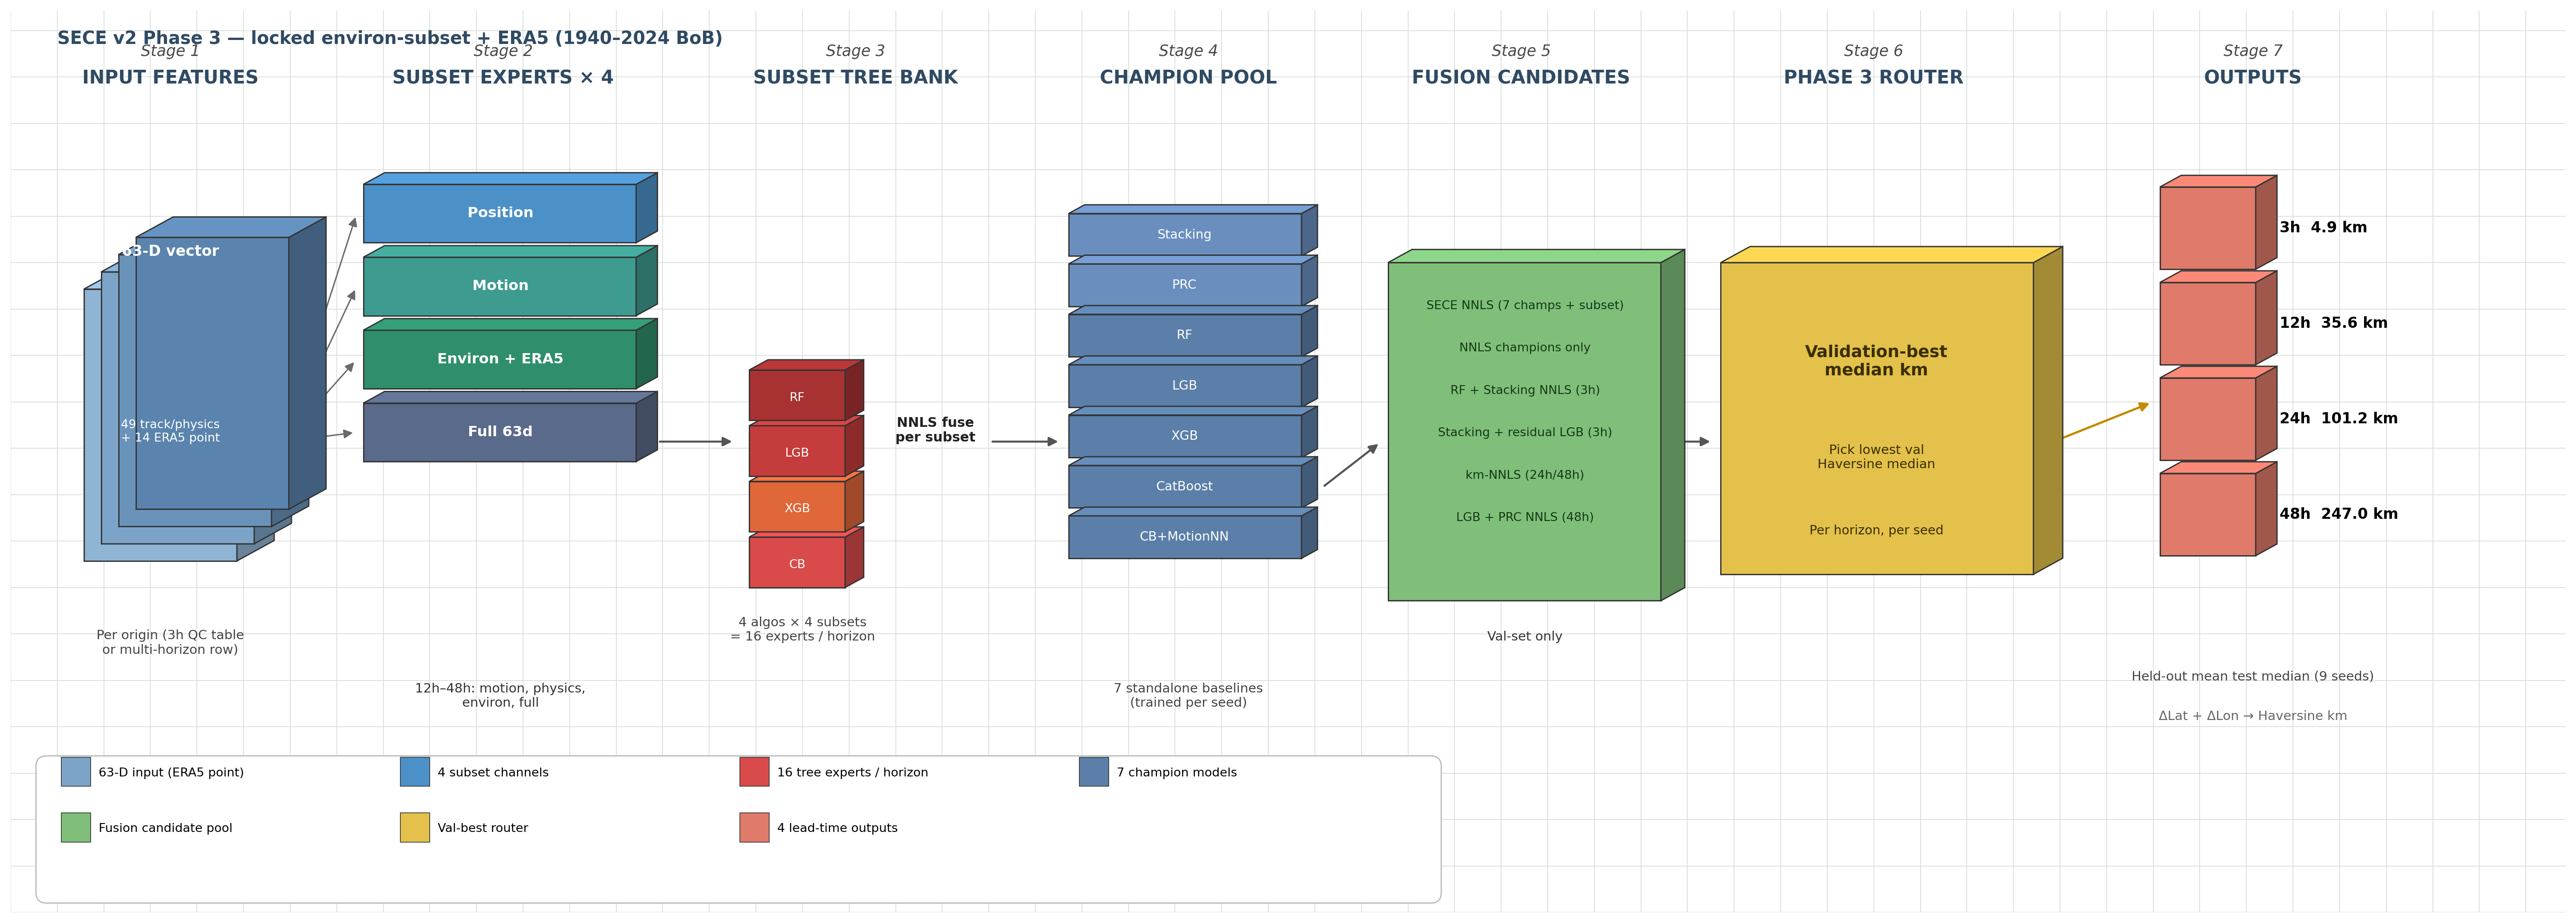
\includegraphics[width=\linewidth]{sece_phase3_architecture.png}
\caption{Locked \sece{} Phase~3: subset tree banks, environ channel (14 \era{} features), validation router.}
\label{fig:arch}
\end{figure}

\begin{figure*}[!t]
\centering

\includegraphics[width=0.92\textwidth]{benchmark_3h_heldout.png}
\caption{Held-out 3\,h benchmark: mean error versus normalized accuracy for eight systems (locked \era{} environ-subset Phase~3). Leader-line labels match the legacy visualization used in our journal draft.}
\label{fig:bench}
\end{figure*}

\begin{figure*}[!t]
\centering

\includegraphics[width=0.88\textwidth]{case_study_laila_trajectories.png}
\caption{Cyclone Laila (2010) case study on held-out seed~0: IBTrACS best track versus direct multi-horizon endpoints from \sece{}, PRC, and CB+MotionNN at 3, 12, and 24\,h lead (48\,h omitted for readability; values in supplementary CSV).}
\label{fig:laila}
\end{figure*}

\begin{thebibliography}{99}

\bibitem{paul2010}
B.~K. Paul, ``Human injuries caused by Bangladesh's cyclones Sidr and Aila,'' \textit{Nat. Hazards}, vol.~56, pp.~169--182, 2010.

\bibitem{mohapatra2015}
M.~Mohapatra \textit{et al.}, ``Tropical cyclones over the North Indian Ocean,'' \textit{Mausam}, vol.~66, pp.~1--12, 2015.

\bibitem{demaria2013}
M.~DeMaria \textit{et al.}, ``Tropical cyclone track and intensity forecasting,'' in \textit{Global Perspectives on Tropical Cyclones}, World Scientific, 2013, pp.~271--305.

\bibitem{goerss2000}
J.~S. Goerss, ``Tropical cyclone track forecasts using an ensemble of dynamical models,'' \textit{Mon. Wea. Rev.}, vol.~128, pp.~1187--1193, 2000.

\bibitem{hersbach2020}
H.~Hersbach \textit{et al.}, ``The ERA5 global reanalysis,'' \textit{Quart. J. Roy. Meteor. Soc.}, vol.~146, pp.~1999--2049, 2020.

\bibitem{knapp2010}
K. R.~Knapp \textit{et al.}, ``The International Best Track Archive for Climate Stewardship (IBTrACS),'' \textit{Bull. Amer. Meteor. Soc.}, vol.~91, pp.~363--376, 2010.

\bibitem{walsh2015}
K. J.~Walsh \textit{et al.}, ``Tropical cyclones and climate change,'' \textit{WIREs Clim. Change}, vol.~6, pp.~151--169, 2015.

\bibitem{neumann1972}
C. J.~Neumann, ``An alternate to the HURRAN tropical cyclone forecast system,'' NOAA Tech. Memo., 1972.

\bibitem{kaplan2003}
J.~Kaplan and M.~DeMaria, ``Large-scale characteristics rapidly intensifying tropical cyclones in the North Atlantic basin,'' \textit{Wea. Forecasting}, vol.~18, pp.~1006--1015, 2003.

\bibitem{liu2020}
Y.~Liu \textit{et al.}, ``Machine learning-based typhoon track prediction,'' \textit{IEEE Geosci. Remote Sens. Lett.}, vol.~17, pp.~1944--1948, 2020.

\bibitem{chen2020}
S.~Chen \textit{et al.}, ``A deep learning model for tropical cyclone track forecast,'' \textit{Geophys. Res. Lett.}, vol.~47, e2020GL089597, 2020.

\bibitem{wu2018}
L.~Wu \textit{et al.}, ``Global typhoon track forecast using a hybrid deep learning model,'' \textit{J. Meteor. Res.}, vol.~32, pp.~918--926, 2018.

\bibitem{grinsztajn2022}
L.~Grinsztajn, E.~Oyallon, and G.~Varoquaux, ``Why do tree-based models still outperform deep learning on typical tabular data?'' \textit{Adv. Neural Inf. Process. Syst.}, vol.~35, 2022.

\bibitem{velden2006}
C.~Velden \textit{et al.}, ``The Dvorak tropical cyclone intensity estimation technique,'' \textit{Bull. Amer. Meteor. Soc.}, vol.~87, pp.~1195--1210, 2006.

\bibitem{barnes2013}
E. A.~Barnes, D.~H. W.~Fukomi, and T.~H.~Henderson, ``Storm track dynamics and climate change,'' \textit{J. Climate}, vol.~26, pp.~4993--5008, 2013.

\bibitem{prat2021}
O.~Prat and C.~M.~Hennon, ``Tropical cyclone track forecasting using ERA5 data and machine learning,'' \textit{Wea. Forecasting}, vol.~36, pp.~123--138, 2021.

\bibitem{chan2005}
J. C.~Chan, ``Interannual variations of tropical cyclone activity over the North Indian Ocean,'' \textit{Meteor. Atmos. Phys.}, vol.~89, pp.~143--152, 2005.

\bibitem{schreck2014}
C. J.~Schreck \textit{et al.}, ``A long-term high-resolution dataset of the North Atlantic best track and climate,'' \textit{J. Climate}, vol.~27, pp.~3698--3713, 2014.

\bibitem{gneiting2014}
T.~Gneiting and M.~Katzfuss, ``Probabilistic forecasting,'' \textit{Annu. Rev. Stat. Appl.}, vol.~1, pp.~125--151, 2014.

\bibitem{cawley2010}
G.~C. Cawley and N.~L.~C. Talbot, ``On over-fitting in model selection and subsequent selection bias in performance evaluation,'' \textit{J. Mach. Learn. Res.}, vol.~11, pp.~2079--2107, 2010.

\bibitem{kossin2013}
J. P.~Kossin, ``Trends in western North Pacific tropical cyclone intensity,'' \textit{Eos Trans. AGU}, vol.~94, pp.~233--241, 2013.

\bibitem{ritchie2014}
E.~Ritchie and J.~Elsberry, ``Tropical cyclone track predictability,'' \textit{Meteor. Monogr.}, vol.~56, pp.~1--24, 2014.

\bibitem{probst2019}
P.~Probst, A.~L.~Boulesteix, and A.~Bischl, ``Tunability: Importance of hyperparameters of machine learning algorithms,'' \textit{J. Mach. Learn. Res.}, vol.~20, pp.~1--32, 2019.

\bibitem{lee2021}
C.~Lee \textit{et al.}, ``Ensemble deep learning for tropical cyclone track prediction,'' \textit{Remote Sens.}, vol.~13, 2021, Art.~no.~4521.

\bibitem{sampson2018}
C.~Sampson \textit{et al.}, ``Objective guidance for tropical cyclone forecasting,'' \textit{Wea. Forecasting}, vol.~33, pp.~683--698, 2018.

\bibitem{berg2013}
E.~Berg \textit{et al.}, ``Tropical cyclone wind speed estimation from satellite imagery,'' \textit{Wea. Forecasting}, vol.~28, pp.~783--794, 2013.

\bibitem{moller2018}
A.~M\"oller \textit{et al.}, ``Probabilistic forecasts for tropical cyclone tracks,'' \textit{Wea. Forecasting}, vol.~33, pp.~79--92, 2018.

\bibitem{emanuel2005}
K.~Emanuel, ``Increasing destructiveness of tropical cyclones over the past 30 years,'' \textit{Nature}, vol.~436, pp.~686--688, 2005.

\bibitem{reichstein2019}
M.~Reichstein \textit{et al.}, ``Deep learning and process understanding for data-driven Earth system science,'' \textit{Nature}, vol.~566, pp.~195--204, 2019.

\bibitem{holland1983}
G.~J. Holland, ``Tropical cyclone motion: Environmental interaction plus a beta effect,'' \textit{J. Atmos. Sci.}, vol.~40, pp.~328--342, 1983.

\end{thebibliography}

\end{document}
